\documentclass[UTF8,12pt, AutoFakeBold,fontset = founder]{ctexart}
% fontset = founder 设置更加丰富的字体
\usepackage{geometry,amsmath,amsthm,amssymb,amsfonts}
\usepackage{graphicx}
\usepackage{float}  % 导入代码块浮点包
\usepackage{microtype} % 解决行溢出问题
\setlength{\emergencystretch}{3em} % 解决行溢出问题


% \setlength{\voffset}{0.6cm} % 将页面内容向上移动

\usepackage{fancyhdr}
\renewcommand{\headrulewidth}{0pt} % 移除页眉横线
% \sectionfont{\centering} % 居中显示标题
\fancyhf{} % 清空当前的页眉和页脚设置
\fancyfoot[C]{\thepage} % 将页码放置在页脚中央

% 定义自定义的页眉页脚样式
% \fancypagestyle{plain}{ % 'plain' 是文档类默认的页面样式
%   \fancyhf{}  % 清空默认的页眉页脚
%   \fancyfoot[C]{\thepage}  % 页脚居中显示页码
% }

\usepackage{sectsty}
\usepackage{authblk} % 对应中文部分的作者机构特殊语法
\usepackage{booktabs}
\usepackage{enumitem}

\usepackage{titletoc}
\usepackage{titlesec}
\usepackage{zhnumber} % 设置标题中文序号
\renewcommand\thesection{\zhnum{section}}
\renewcommand\thesubsection{\arabic{section}.\arabic{subsection}}

\usepackage{tocloft} % 用于定制目录中的条目格式

% 重定义目录标题
\renewcommand{\contentsname}{%
  \fontsize{16pt}{24pt}\selectfont % 三号字体,1.5 倍行距
  \bfseries 目录 % 加粗
  \vspace{24pt} % 段前 24 磅
}

% % 设置目录中章节标题的格式
% \titlecontents{section}
%   [0em] % 左边距
%   {\bfseries \songti \fontsize{11pt}{13pt}\selectfont} % 标题格式
%   {\contentslabel{0.9em}{、}} % 标签格式(序号和顿号)
%   {}
%   {\titlerule*{.}\contentspage}

% % 设置目录中二级标题格式
% \titleformat{\subsection}
%   {\songti \fontsize{12pt}{18pt}\selectfont} % 宋体、小四号
%   {\thesubsection} % 编号
%   {0em} % 编号与标题之间的水平间距
%   {} % 标题内容前的附加内容
%   [\vspace{0pt}] % 段后 0 磅

% % 设置目录中三级标题格式
% \titleformat{\subsubsection}
%   {\songti \fontsize{12pt}{18pt}\selectfont} % 宋体、小四号
%   {\thesubsubsection} % 编号
%   {0em} % 编号与标题之间的水平间距
%   {} % 标题内容前的附加内容
%   [\vspace{0pt}] % 段后  0 磅


\CTEXsetup[name={第,章},number={{\arabic{section}}}]{section}
\sectionfont{\centering} % 居中显示标题

% 使用 titlesec 设置章节与标题的分隔符
% 自定义带编号章节格式:第x章 标题(居中)
\titleformat{\section}[block]{\centering\bfseries\large}{第\arabic{section}章\quad}{0pt}{}

% 自定义无编号章节格式(摘要/参考文献/致谢)
\titleformat{name=\section,numberless}[block]{\centering\bfseries\large}{}{0pt}{}

% 禁用默认标题
% \renewcommand{\refname}

% 设置 subsection 格式
\titleformat{\subsection}
  {\mdseries \heiti \fontsize{12pt}{18pt}\selectfont} % 黑体、小四号、加粗
  {\thesubsection} % 编号
  {1em} % 编号与标题之间的水平间距
  {} % 标题内容前的附加内容
%   [\vspace{0.5em}] % 标题后的垂直间距

% 设置 subsubsection 格式
\titleformat{\subsubsection}
  {\mdseries \heiti \fontsize{12pt}{18pt}\selectfont} % 黑体、小四号、加粗
  {\thesubsubsection} % 编号
  {1em} % 编号与标题之间的水平间距
  {} % 标题内容前的附加内容
%   [\vspace{0.5em}] % 标题后的垂直间距

% \CTEXsetup[name={\heiti \fontsize{14.4pt}{21pt}\selectfont},number={}]{section}

% \CTEXsetup[format={\Large\bfseries}]{section}

\setlength{\baselineskip}{20pt}  % 正文20磅行距

\newcommand{\wideword}[1]{%
  \sodef\spaced{}{0.07cm}{0.07cm}{0.07cm}%
  \spaced{#1}%
}

\usepackage{listings} % 配置附件代码块
\usepackage{setspace}
\usepackage{ragged2e} % 设置两端对齐需要的模块
\newcommand{\sectspacemode}{\setstretch{1.5}} % 设置\section内容的行距为1.5倍

\usepackage{hyperref} % 点击跳转
\usepackage{xcolor} % 引入颜色包
\usepackage{caption}
\usepackage{subcaption} % 引入子图
\usepackage{extsizes} % 扩展字体,允许使用字号更大

\hypersetup{hidelinks,
	colorlinks=true,
	linkcolor=black,  % 目录链接的颜色
    citecolor=blue,  % 文献引用的链接颜色
	pdfstartview=Fit,
	breaklinks=true
}

%! 下面这条命令是不压缩pdf, 这样编译tex会很快,但是最终的pdf会很大,如果最终定稿了,请注释掉此行,这样最终的pdf会更小
\special{dvipdfmx:config z 0}

% 设置图、表、公式
\counterwithin{figure}{section}
\renewcommand{\figurename}{Figure} % 将图变成figure
\counterwithin{table}{section}
\renewcommand{\tablename}{Table}
\counterwithin{equation}{section}

\renewcommand{\thefigure}{\arabic{section}.\arabic{figure}}
\renewcommand {\thetable} {\arabic{section}.\arabic{table}}
\renewcommand {\theequation} {\arabic{section}.\arabic{equation}}

\captionsetup{labelformat=default,labelsep=space} %去除图注、表注的冒号
% 设置图像图注为中文
\captionsetup[figure]{name=图}
\graphicspath{{../images/}} % 设置图片路径
% 设置表格图注为中文
\captionsetup[table]{name=表}

% 作者格式
% \renewcommand*{\Authsep}{,}
% \renewcommand*{\Authand}{,}
% \renewcommand*{\Authands}{,}

\geometry{paperwidth=21cm, paperheight=29.7cm,left=3cm,right=3cm,top=2.5cm, bottom=2.5cm}

% 设置中文字体为宋体
\setCJKmainfont{SimSun}

% 设置英文字体为 Times New Roman
\setmainfont{Times New Roman}
% 引入华文行楷字体
\setCJKfamilyfont{huawenxingkai}{STXingkai} % 字体名称可能与系统显示不同,需确认
\newcommand{\huawenxingkai}{\CJKfamily{huawenxingkai}}

% 设置段落格式
\setlength{\parindent}{2em} % 首行缩进 2 字符
\setlength{\parskip}{0pt} % 段前段后 0 磅
\linespread{1.08} % 行距 20 磅(12pt × 1.08 ≈ 20pt)
\justifying % 两端对齐

% \title{Prediction of urban air quality by data mining}
% % authblk 提供的特殊用法,将作者机构作为 option 进行捆绑
% \author[1]{Long Liu}
% \affil{School of Information Engineering}
% \date{}
\usepackage{subfiles} % 多文件编译包
\usepackage{cite}

\bibliographystyle{ref/gbt7714-numerical}

\begin{document}
% \begin{sloppypar}
\makeatletter
% 定义引用格式
\def\@cite#1#2{\textsuperscript{[{#1\if@tempswa , #2\fi}]}}
\setlist[enumerate]{itemsep=0pt, parsep=0pt} % 设置enumerate环境的垂直间距

\subfile{sections/cover}

\subfile{sections/abstract}



\pagestyle{fancy} % 从这个地方一下全遵循自定义页眉
\newpage
% 添加目录
% \pagenumbering{Roman} % 使用小写罗马数字作为目录页码
% \setcounter{page}{1} % 重置页码计数器
\begin{flushleft}
    \phantomsection % 手动插入锚点
    \centering\tableofcontents
    \addcontentsline{toc}{section}{目录} % 将“目录”添加到目录
\end{flushleft}


\clearpage
\pagenumbering{arabic} % 切换到阿拉伯数字作为正文页码
\setcounter{page}{1} % 重置页码计数器
% 通常来说,你在下面章节填充内容即可!
\subfile{sections/section1-Introduction}

% \subsection{数据集}

% 表格识别技术的发展离不开高质量数据集的支持,这些数据集为研究者提供了多样化的训练样本,推动了表格识别算法的进步。多个经典数据集为该领域提供了重要的基础。例如,UW-3\cite{data1}(1996年)数据集包含1600张经过倾斜校正的英文文档图像,奠定了表格识别的早期基础;UNLV\cite{data1}(2012年)和Marmot\cite{data1}(2012年)数据集提供了大量扫描文档图像和实体边界框,涵盖了不同类型和布局的表格;ICDAR 2013、ICDAR 2015\cite{data2}和ICDAR 2017\cite{data3}数据集作为表格识别领域的基准数据集,广泛应用于表格检测与结构识别竞赛。随着研究的深入,DeepFigures\cite{data5}(2018年)和ICDAR 2019\cite{data4}(2019年)等数据集相继发布,进一步丰富了表格识别的研究样本,支持表格检测和结构识别任务。PubTabNet\cite{data6}(2020年)和TableBank\cite{data7}(2020年)则为表格检测和结构识别提供了大量HTML格式的表格数据,推动了数据驱动的表格识别技术的发展。SciTSR\cite{data8}(2019年)和FinTab\cite{data9}(2021年)则专注于特定领域,如科学论文和财务表格,提供了多样化的标注数据。此外,WTW\cite{data10}(2021年)数据集专注于自然场景下的表格数据,特别针对图像的扭曲、倾斜等失真问题,提供了形变表格识别的重要数据支持,推动了该领域的进展。最新发布的PubTables-1M\cite{data11}(2022年)和TabRecSet\cite{data12}(2022年)数据集为端到端表格识别提供了大量样本,涵盖了多种语言和表格类型,进一步扩展了表格识别技术的应用范围。WikiTableSet\cite{data13}(2023年)包含近400万张英文、日文和法文表格图像,为跨语言的表格识别研究提供了重要的数据支持。这些数据集的发布为表格识别技术的发展提供了重要的数据支撑,推动了表格识别算法的进步,并为未来的研究提供了宝贵的资源。

\section{预期目标}

通过对本文提出的问题的研究,结合现有的表格识别方法,预期达到以下目标:

对于存在形变的有网格线表格图像,设计并实现一种基于深度学习的图像分割方法,尽最大可能识别和分割表格中每个单元格的细粒度的坐标,此外,本课题还将设计一种算法,用于确定单元格之间的相对位置,能获取单元格在表格中行、列以及合并信息。

\subfile{sections/section2-.tex}

\section{研究方案}
\subsection{数据集的构建}
\subsection{单元格逻辑坐标定位}

单元格逻辑坐标的定位是表格结构识别中的关键步骤之一。其基本思路是通过分析相邻关系,识别所有属于同一行或同一列的单元格,并将这些单元格归入相应的集合中。对于非跨行单元格,它只能出现在一个行集合中;而对于跨行单元格,则可以出现在多个行集合中,以表示该单元格跨越的行范围。列集合同理。为了解决判断相邻关系这一关键问题,本文提出了两个概念:最短基准投影重叠率和质心扩展矩形。

\subsubsection{最短基准投影重叠率}
首先,为了判断单元格是否相邻,需要引入最短基准投影重叠率(Minimum Projection Overlap Ratio,MPoR)来判断某个方向上线的同属程度,设两条线段 \( L_1 \) 和 \( L_2 \),它们在指定方向上的投影区间为 \([a_1, b_1]\) 和 \([a_2, b_2]\),则最短基准投影重叠率定义为:
\begin{equation}
    \mathcal{P}(L_1,L_2) = \frac{\min(b_1, b_2) - \max(a_1, a_2)}{min(b1-a1, b2-a2)}
\label{eq:piol}
\end{equation}


其中$\min(b_1, b_2) - \max(a_1, a_2)$实际上就是投影的重叠长度(如果出现负数,那么说明在该方向上是没有重叠的,两条线之间也就没有同属关系)。

通过单元格的边界线段判断单元格是否在y轴方向上是否隶属同一行或者x轴方向上是否隶属同一列(后文如果没有强调,这里使用的都是两个矩形相邻的边计算MPoR值)。

\begin{figure}[H]
    \centering
    % 第一个子图
    \begin{subfigure}[b]{0.3\textwidth}
        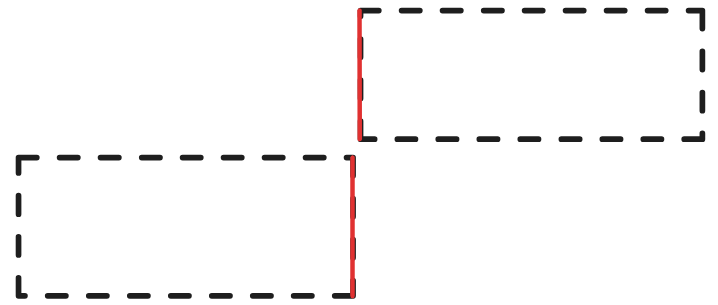
\includegraphics[width=\textwidth]{../images/a.png}
        \caption{不属于同一行}
        \label{fig:a}
    \end{subfigure}
    \hfill
    % 第二个子图
    \begin{subfigure}[b]{0.3\textwidth}
        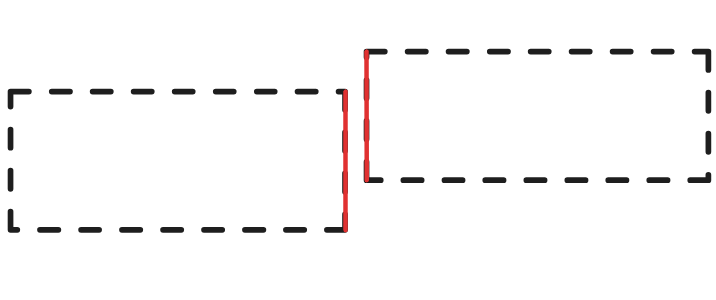
\includegraphics[width=\textwidth]{../images/b.png}
        \caption{属于同一行}
        \label{fig:b}
    \end{subfigure}
    \hfill
    % 第三个子图
    \begin{subfigure}[b]{0.3\textwidth}
        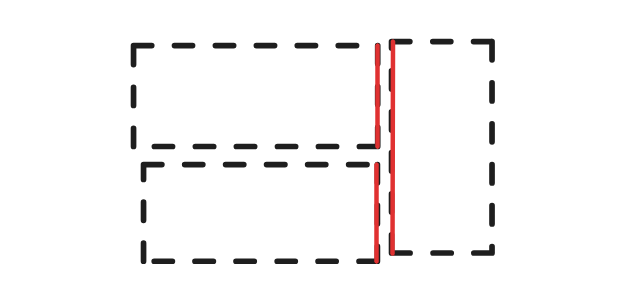
\includegraphics[width=\textwidth]{../images/c.png}
        \caption{合并行情况}
        \label{fig:c}
    \end{subfigure}
    \captionsetup{labelsep=colon} 
    \caption{(\subref{fig:a})是左右两个矩形在水平方向的MPoR值小于给定的阈值t,所以可以判定不属于同一行,(\subref{fig:b})是左右两个矩形在水平方向的MPoR值大于给定的阈值t,所以可以判定属于同一行,(\subref{fig:c})是左边两个矩形与右边矩形在水平方向的MPoR值均大于给定的阈值t,所以可以判定右边的矩形是合并单元格,并且既属于左上矩形所在行又属于左下矩形所在行}
\end{figure}

\subsubsection{质心扩展矩形}

实例分割的轮廓是复杂的掩码,为了更加方便的确定单元格的逻辑坐标,需要引入质心扩展矩形(Centroid-Expansion Rectangle,CER)来简化掩码,首先计算掩码的质心,通过质心向上下左右四个方向扩展,计算质心四个方向的射线与轮廓的交点,于是就会得到掩码在垂直高度与水平宽度上的参考值,结合宽高和质心可以得到质心扩展矩形,如图\ref{fig:r}(\subref{fig:CER}),质心扩展矩形的宽高具有参考作用,但是也会存在误差,所以最终参考的的垂直范围和水平范围是通过修正的,具体的修正方式如图\ref{fig:r}(\subref{fig:h-re})和\ref{fig:r}(\subref{fig:w-re})所示,将质心的四边界向内(质心方向)收缩$\delta $个像素,并计算收缩后的四边界所在位置的延长线被轮廓所截取的范围,修正之后的高度范围选取左右截取范围的最大值,修正之后的宽度范围选取上下截取范围的最大值。

\begin{figure}[H]
    \centering
    % 第一个子图
    \begin{subfigure}[b]{0.3\textwidth}
        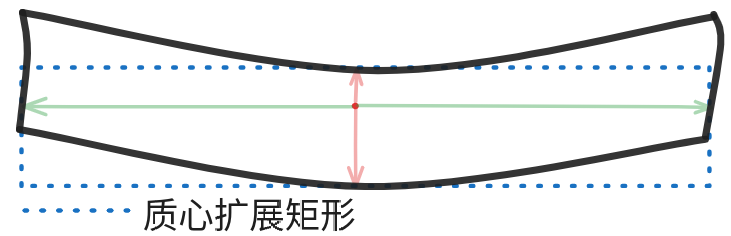
\includegraphics[width=\textwidth]{../images/CER.png}
        \caption{质心扩展矩形}
        \label{fig:CER}
    \end{subfigure}
    \hfill
    % 第二个子图
    \begin{subfigure}[b]{0.3\textwidth}
        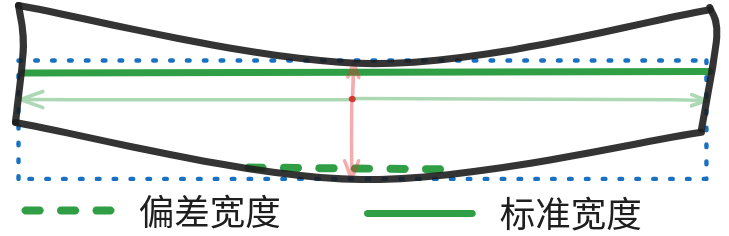
\includegraphics[width=\textwidth]{../images/x.png}
        \caption{修正宽度}
        \label{fig:w-re}
    \end{subfigure}
    \hfill
    % 第三个子图
    \begin{subfigure}[b]{0.3\textwidth}
        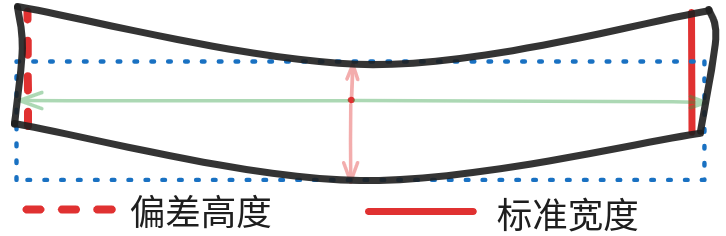
\includegraphics[width=\textwidth]{../images/y.png}
        \caption{修正高度}
        \label{fig:h-re}
    \end{subfigure}
    \caption{质心扩展矩形}
    \label{fig:r}
\end{figure}


\subsubsection{基于分治思路的单元格行列划分}

\section{拟解决的关键问题与创新点}

\section{研究计划进度}

% 参考文献部分
\clearpage
\phantomsection % 手动插入锚点
\addcontentsline{toc}{section}{参考文献}
\bibliography{ref/ref}

\clearpage
\phantomsection % 手动插入锚点
\section*{攻读硕士期间发表论文及参加科研情况}
\addcontentsline{toc}{section}{攻读硕士期间发表论文及参加科研情况}
这里写科研成果

\clearpage
\phantomsection % 手动插入锚点
\section*{致谢}
\addcontentsline{toc}{section}{致谢}
这里写致谢

{
\newpage
\thispagestyle{empty}
\newgeometry{paperwidth=21cm, paperheight=29.7cm, left=3cm,right=3cm,top=2.5cm, bottom=2.5cm}
\thispagestyle{empty}

\begin{center}
    \vspace{21.6pt}
     {\fontsize{18}{21.6}\selectfont\heiti  南昌航空大学硕士学位论文原创性声明}
\end{center}
\vspace{12.6pt}
\begin{spacing}{1.9}
\zihao{4}
本人郑重声明:所呈交的硕士学位论文,是我个人在导师指导下,在南昌航空大学攻读硕士学位期间独立进行研究工作所取得的成果。尽我所知,论文中除已注明部分外不包含他人已发表或撰写过的研究成果。对本文的研究工作做出重要贡献的个人和集体,均已在文中作了明确地说明并表示了谢意。本声明的法律结果将完全由本人承担。
\end{spacing}

\vspace{16.8pt}
{\zihao{4} 签名:\underline{\hspace{5cm}} \hspace{1cm} 日期:\underline{\hspace{5cm}}}

\vspace{34.2pt}

\begin{center}
    {\fontsize{18}{21.6}\selectfont\heiti  南昌航空大学硕士学位论文使用授权书}
\end{center}
\vspace{16.8pt}
\begin{spacing}{1.9}
\zihao{4}
本论文的研究成果归南昌航空大学所有,本论文的研究内容不得
以其它单位的名义发表。本人完全了解南昌航空大学关于保存、使用
学位论文的规定,同意学校保留并向有关部门送交论文的复印件和电
子版本,允许论文被查阅和借阅。本人授权南昌航空大学,可以采用
影印、缩印或其他复制手段保存论文,可以公布论文的全部或部分内容。同时授权中国科学技术信息研究所将本学位论文收录到《中国学位论文全文数据库》,并通过网络向社会公众提供信息服务。
\end{spacing}

{\zihao{4}(保密的学位论文在解密后适用本授权书)}

\vspace{16.8pt}
{\zihao{4} \noindent
签名:\underline{\hspace{3cm}} 导师签名:\underline{\hspace{3cm}} 日期:\underline{\hspace{3cm}}}

}
% \end{sloppypar}
\end{document}

